\subsection{Periodic Background Tasks}\label{ssec:periodictasks}
When the app is installed the program needs to run a task periodically to collect location data.
\Citet{friesen2015android} writes how this can be done in the Android API with respectively the AlarmManager and the JobSchedular.

\paragraph{AlarmManager}
In the first Android version (API 1) the AlarmManager was created to handle alarms.
They implemented it as a general class which can call any task after a given period has passed.
The alarm can then be set to be reoccurring which means that we can use this to cache location data in a set interval.

\paragraph{JobScheduler}
In Android 5.0 (API 21) an alternative to the AlarmManager was implemented, the JobScheduler.
This functions in a similar way as the AlarmManager, but tries to batch the jobs together and execute them in bundles.
This means that the device can save power by avoiding going to sleep just to wake a short moment later.
The sacrifice for this is precision in time. 
While the AlarmManager has the option to occur at a exact time, the JobSchedular does not.
This is needed to give the JobScheduler enough control to efficiently batch the jobs together.

Because the timing of the location data is less important than the constant stream of data the JobScheduler is chosen as the basic for the background tasks.
This has the advantages of saving power which is preferable.

\subsection{Location tracking}\label{ssec:loctrack}
% metatext
In order to be able to locate a user and to construct routes, it is necessary to collect location data. 
The location data should only be collected when the user is driving in a vehicle. 
Such collection of location data can be done by using already existing services, such as the Google Play Service.

% something
Location data in \gls{rs} is only useful if it is formatted in GPS coordinates, stored in a collection that represents a route from A to B.
There are several ways to collect location data. 
One of them is by developing a component to do so on the android device. 
Another way is to use already existing services, such as one of the Google Play Services.


To use Google Play Services, a client library must be included in the app, which will communicate via inter-process communication to the Google Play Services which is already existing on every android device. 
When the application is connected to the Google Play Services \cite{GapiOverview}, it will automatically receive silent updates regularly, to acquire new features and bug fixes to the used services. 
This is illustrated in Figure \ref{fig:gapifigure}.

\begin{figure}[h]
	\centering
	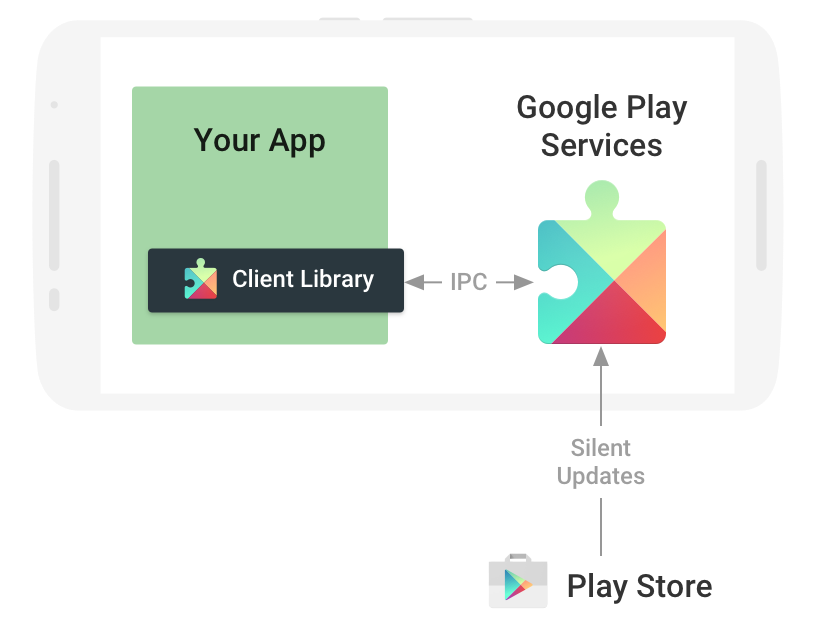
\includegraphics[width=0.7\textwidth]{figures/play-services-diagram.png}
	\caption{Google Play Services communication\cite{GapiFigure}}
	\label{fig:gapifigure}
\end{figure}

The Google Play Services are restricted, and are not supporting devices with Android versions lower than 2.3. 
This limits the backwards compatibility, but the app is already restricted to Android 5 and newer, and has no influence on the target audience.

The Google Play Services will allow the application to collect location data, but it is not doing so solely using the GPS in the device. 
The location service utilizes both network location and GPS to estimate a position as precise as possible \cite{GapiLocation}. 
To ensure the collected location data is relevant, it is needed to store data only when the user is traveling by vehicle.
The Google Play Services provides a service to determine the user's activity, called Activity recognition. 

Activity recognition is a service that uses several sensors on the device to determine what kind of activity the user is currently performing, therein driving, walking, etc.
The service will return a probability level from 1 to 100, where 100 is certain that a user is performing the activity.
The activity recognition will be used to prevent unnecessary data will be stored on the database. 


The piratical design of the location tracking and activity recognition will be further explored in the following design section.

As external tools are examined a look at the \gls{astep} system and what it will have to offer is discussed.